\documentclass[10pt,a4paper]{report}
\usepackage[utf8]{inputenc}
\usepackage[english]{babel}
\usepackage[T1]{fontenc}
\usepackage{amsmath}
\usepackage{amsfonts}
\usepackage{graphicx}
\usepackage{lmodern}
\usepackage{amssymb}
\usepackage{verbatim}
\usepackage{float}
\usepackage{minitoc}
\usepackage{amsthm}
\newtheorem{definition}{Definição}
\newtheorem{theorem}{Teorema}
\usepackage{hyperref}
\title{\LARGE{Network and Computer Security } \\ \vspace{0.5cm} \normalsize{Summary}}
\date{}

\begin{document}
\maketitle
\tableofcontents

\chapter{Cryptography}
It is a widespread and dangerous belief that encrypting everything provides protection against anything. In reality, when the algorithm is known it is necessary to prevent several types of attacks, such as ciphertext-only, known-plaintext, chosen-plaintext or chosen-ciphertext. Cryptography must, then, protect the information against unauthorized insertion of information, modification of information in transit, replay of information and access to information.
\section{Cryptographic Services}
To this end, we need the following cryptographic services:
\begin{itemize}
\item Confidentiality: a service used to keep the content of the information from all, but those entities authorized to have it. Has the drawbacks of making debugging harder and may lead to information loss if the key is lost. Can be assured through symmetric of assymetric cipher.
\item Integrity: a service that detects data manipulation by unauthorized entities (not the same thing as error detection codes). An intruder should not be able to substitute a false message for a legitimate one. Can be assured through MIC or a digital signature.
\item Authenticity: a service used to ascertain the identity or the origin of a message. Can be assured through MIC or a digital signature, tough freshness requires adding a nonce to the message.
\begin{itemize}
\item Entity authentication: verify the identity of an entity
\item Data origin authentication: confirm the creator of the message
\item Non-repudiation: a service which prevents an entity from denying. Can be assured by a digital signature.
previous commitments or actions
\end{itemize}
\end{itemize}
\section{Cryptographic Building Blocks}
\subsection{Symmetric Cipher}
Uses the same key to cipher and decipher. In cryptographic function notation:
\begin{itemize}
\item $E(M,K)$: cipher message $M$ with key $K$
\item $D(C,K)$: decipher cryptogram $C$ with key $K$
\end{itemize}
\subsection{Asymmetric Cipher}
A public/private pair of keys is used ($KU/KR$). In cryptographic function notation:
\begin{itemize}
\item $AE(M, KR)$: cipher message $M$ with private key $KR$
\item $AD(C, KU)$: decipher cryptogram $C$ with public key $KU$
\end{itemize}
It is also possible to cipher with the public key and then decipher with the private key.
\subsection{Cryptographic Hash}
A cryptographic hash function does not use a key, instead receives an input message and returns a digest of the data. In cryptographic function notation:
\begin{itemize}
\item $H(M)$: hash of message $M$
\end{itemize}
The digest value is deterministic, has fixed size, a unique representation, is non-reversible and sensible to input changes.
\subsection{Composite Building Blocks}
\begin{itemize}
\item Hybrid cipher: a random symmetric key is generated and used to cipher the message. This key is then ciphered with the public key of the receiver and is sent along with the ciphered message. The receiver must decipher the symmetric key with its private key and use it do decipher the message
\item Message integrity code: the MIC is created by creating the digest of the message and ciphering the result. It can then be used to check the integrity of the message by generating a new hash and comparing to the sent one.
\item Digital signature: a digital signature is created by ciphering a digest with the private key. The receiver can then decipher with the public key and verify the identity of the sender.
\end{itemize}
\section{Symmetric Criptography}
Symmetric ciphers use a single secret key that may be shared by 2 or more communicating parties. This allows confidentiality to all those who have the key and message authentication, with good performance. The main problem lies in key distribution\\
\\
For $N$ communicating parties, $N \times (N-1) / 2$ keys are needed for them to be able to communicate 1 - 1 secretly.\\
\\
An example of a symmetric cipher is the one-time pad, where the message is XOR'd with the key. The security is based on the assumption that the key is never reused.
\subsection{Symmetric Stream Ciphers}
Symmetric stream ciphers are pratical approximations to the one-time pad. Keystreams are generated in a deterministic way from a fixed size key (approximation to real random sequence generators).
\begin{figure}[H]
\centering
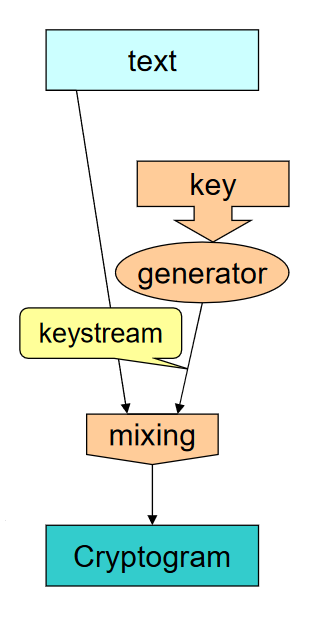
\includegraphics[scale=0.4]{1.png}
\end{figure}
In this type of cipher, if the plain text is known, the keystream is exposed. The secure pseudo-random generators are sometimes based on LFSRs (Linear Feedback Shift Registers). It consists on a state machine that produces a cyclic sequence of bits:
\begin{figure}[H]
\centering
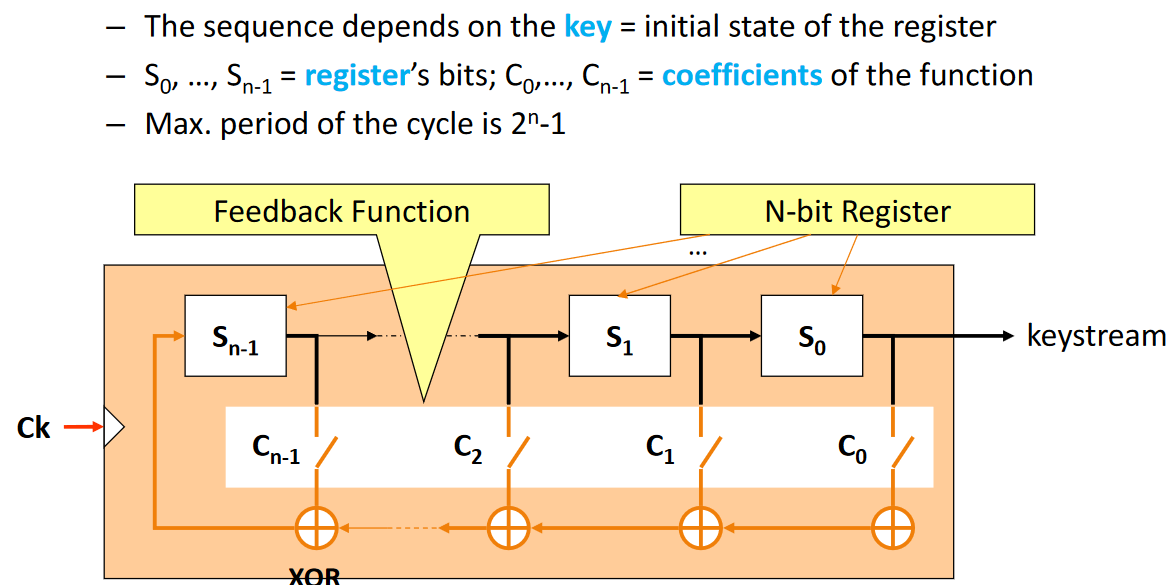
\includegraphics[scale=0.4]{2.png}
\end{figure}
\subsection{Symmetric Block Ciphers}
These are also  based on approximations, using Shannon’s notions of confusion (repeated application of a complex function to a large block) and diffusion (permutation, substitution, expansion and compression).
\subsubsection{Feistel Network}
The feistel network is a complex  function most commonly
used in block cipher algorithms. It applies a round function $F$ over multiple rounds:
\begin{itemize}
\item Each round uses a different round key ($K_i$), obtained from the key ($K$)
\item Text is split in left (L) and right (R) parts
\end{itemize}
The cipher and decipher processes are the same, with the keys used in the inverse order.
\begin{figure}[H]
\centering
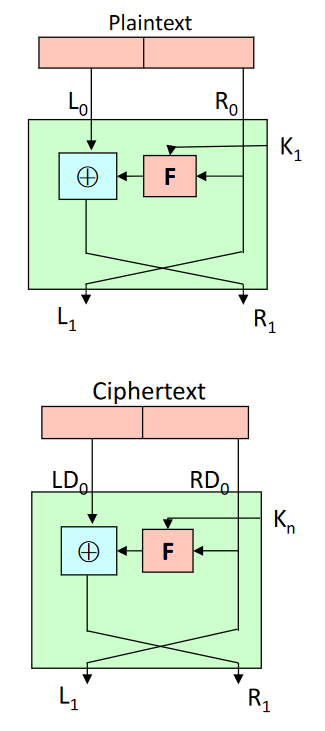
\includegraphics[scale=0.4]{3.png}
\end{figure}
\subsubsection{DES}
The DES algorithm uses 64 bit blocks with 56 bit keys. It applies the feistel network algorithm on several rounds, after an initial permutation of the 64 bits, according to a fixed table.
\subsubsection{Block Cipher Modes}
When using a plaintext of different size than the block, a cipher mode must be used.
\begin{itemize}
\item $Electronic$ $Code$ $Book$ (ECB)
\begin{itemize}
\item Encryption using independent blocks
\item Weakness in reproducing patterns from the original text; identical blocks produce the same ciphertext
\end{itemize}
\begin{figure}[H]
\centering
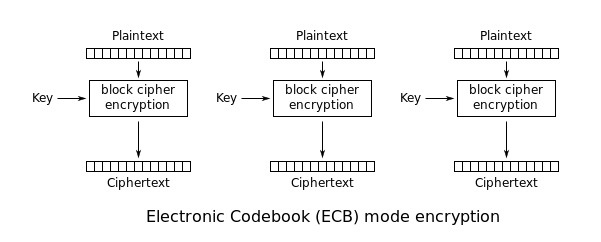
\includegraphics[scale=0.5]{4.png}
\end{figure}
\item $Cipher$ $Block$ $Chaining$ (CBC)
\begin{itemize}
\item Plaintext is XORed with the ciphertext of the previous block before encryption
\item Reduces the risk of pattern replication
\item Uses an initialization vector in the first block (necessary for decryption) and requires padding: bits to compose entire blocks of the size required by the algorithm
\end{itemize}
\begin{figure}[H]
\centering
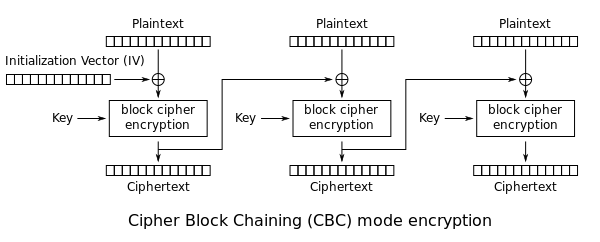
\includegraphics[scale=0.5]{5.png}
\end{figure}
\item $Output$ $Feedback$ (OFB)
\begin{itemize}
\item Retains the advantages of CFB, and the ciphertext is not used in the next block, allowing block cipher operations to be performed in advance, enabling parallel XOR as soon as the text (plaintext or ciphertext) is available
\end{itemize}
\begin{figure}[H]
\centering
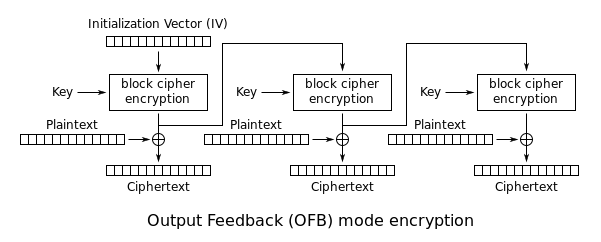
\includegraphics[scale=0.5]{6.png}
\end{figure}
\item $Counter$ $Mode$ (CTR)
\begin{itemize}
\item Standard cipher mode in AES
\item Uses a nonce and a counter, which must be different in each cipher operation
\end{itemize}
\begin{figure}[H]
\centering
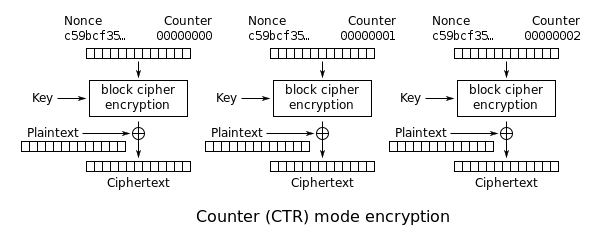
\includegraphics[scale=0.5]{7.png}
\end{figure}
\item $Galois$ $Counter$ $Mode$ (GCM)
\begin{figure} [H]
\centering
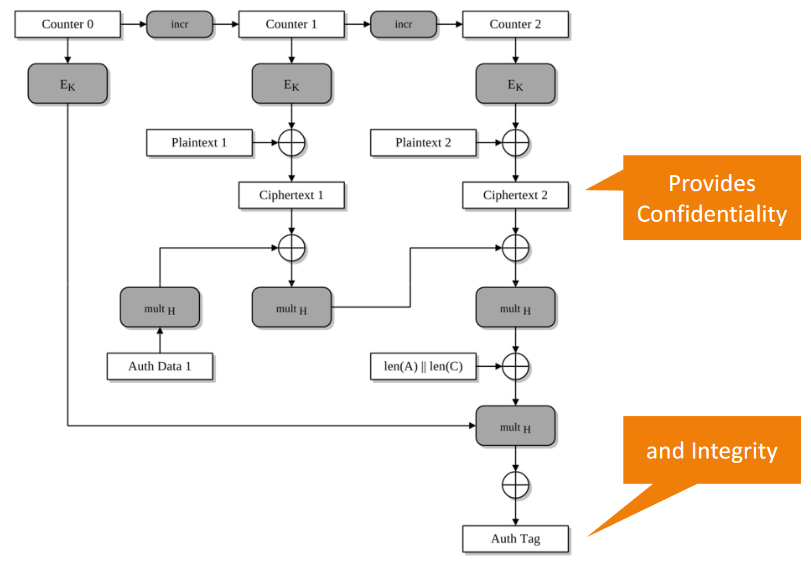
\includegraphics[scale=0.4]{8.png}
\end{figure}
\end{itemize}
\subsubsection{Padding}
Sometimes it may be necessary to pad the last block, when the message size is not divisible by the block length. This may be done by:
\begin{itemize}
\item Padding with zero (null) bytes, spaces (0x20), all bytes of the same value
\item Padding with random bits
\item Padding with 0x80 (1000 0000) followed by zero (null) characters
\item Padding with the PKCS\#5 scheme: Sequence of bytes, each of which equal to the number of padding bytes (e.g.   if 24 bits of padding need to be added, the padding string is "03 03 03": 3 bytes times 8 bits equals 24)
\end{itemize}
\subsubsection{AES}
AES is the current encryption standard. Supports keys of 128, 192 and 256 bits with 128 bit blocks. It runs in 10, 12 or 14 rounds, in which it substitutes bytes, shifts rows, mixes columns and adds the round key XOR state with key material)
\section{Hash Functions}
These are cryptagraphic functions, but not ciphers. They must be:
\begin{itemize}
\item Collision resistance: Computationally infeasible to find two inputs that give the same hash
\item Preimage resistance: Given a hash, it’s computationally infeasible to find an input that produces that hash
\item Seconde preimage resistant: Given a hash value and the corresponding input, it’s computationally infeasible to find a second input that generates that same hash
\end{itemize}
The most common algorithms are:
\begin{itemize}
\item MD5 (128 bits): very weak
\item SHA-1 (160 bits): weak
\item SHA-2 (256 to 512 bits)
\item SHA-3 (256 to 512 bits)
\end{itemize}
Attacks on hash functions are sometimes done by brute force ($P(collision) = 2^{m-1}$) and most often through the birthday attack ( pick $M$, $M'$, $M''$, $M'''$... and obtain hashes until any 2 are identical) ($P(collision) = 2^{m/2}$).
\subsection{Message Integrity Codes}
The objective is to detect changes to a message. It allows the checking of a message's integrity and, with freshness can provide authenticity, thus, it's sometimes called MAC.\\
\\
Under the assumption that the sender and recipient have a shared secret key $K$, the idea is to send the messgae and the MAC; if the message (or the MAC) is modified by an attacker, the recipient will be able to detect it. Attacker cannot create a valid MIC because he does not have $K$.\\
\\
Implementations of MAC could be as follows:
\begin{itemize}
\item Hash the message and encrypt the digest
\item Using a keyed-function (CMAC, usually with CBC)
\item Using a keyed-hash (HMAC)
\end{itemize}
\section{Asymmetric Ciphers}
Asymmetric cryptography uses a pair of public/private keys. It allows for confidentiality, authentication and integrity (digital signatures). Has the advantage of only needing $N$ key pairs, but the performance is much worse.\\
\\
For confidentiality, the public key is used to cipher and the private to decipher. For authentication it's the opposite.
\subsection{One-way Functions}
Also known as trapdoor functions. The idea is for the function to be easy to compute in one direction, but hard to invert. These are usually used in asymmetric cryptography.
\subsection{Algorithms}
\subsubsection{RSA}
In this algorithm, the plaintext is divided into blocks, which are treated as a number. The keys are generated as follows:
\begin{itemize}
\item Choose two prime numbers $p$ and $q$
\item Define $n = pq$ and $z = \phi(n) = (p-1)(q-1)$
\item Choose $e < n$ such that $e$ is coprime with $z$
\item Calculate $d$ such that $ed \mod z = 1$
\item The public key is $K_u = (e, n)$, and the private key is $K_r = (d, n)$
\end{itemize}
To encrypt, compute:
$$
E(K_u, m) = m^e \mod n = c
$$
And to decrypt:
$$
D(K_r, c) = c^d \mod n = m
$$
RSA is often used to produce signatures. To sign $M$ we calculate $S = (hash(M))^d \mod n$ and to verify we check $hash(M) == S^e \mod n$. Only the owner of the private key can sign, but anyone with the public key can verify the signature.
\subsubsection{ECC}
Elliptic curve cryptography offers the same security as RSA with smaller bit sizes. In this case, the "hard" problem is the elliptic curve logarithm:
\begin{itemize}
\item $Q = k \cdot P$, where $Q, P$ belong to an elliptic curve (e.g. $y^2 = x^3 - 3x + b \mod p$)
\item Easy to compute $Q$, given $k$ and $P$
\item Hard to find $k$, given $Q$ and $P$
\item $P$ is a base point (parameter of the curve)
\end{itemize}
\subsection{Digital Signatures}
Digital signatures use an asymmetric cipher and a hash function. The basic algorithm is as follows:
\begin{itemize}
\item Sign: $S(doc) = E(K_r, hash(doc))$
\item Validate: $D(K_u, S(doc)) == hash(doc)$
\end{itemize}
Today often ECDSA is adopted (with elliptic curve encryption).

\end{document}

%next: 4a